%-----------------------------------------------------------------------------------------

\section{Introduction}
%-----------------------------------------------------------------------------------------

\subsection{Motivation and Context}

Machine Learning algorithms have become ubiquitous in modern life. They power
social media feeds, advertising personalisation and even identifying breast
cancer more accurately than doctors. \cite{Mammograms2020} To train these
Machine Learning algorithms large datasets are needed. The greater the available
data, the more nuanced and accurate the produced model will be.
\par

As the scale of problems we are trying to solve dramatically increases, the
scale of datasets are too. Services like the Internet Archive as of 2020 contain
over 70PB in it's database. Labeled datasets such as AViD have video data in the
order of terabytes. \cite{piergiovanni2020avid} Since 2008 Google has been
processing more 20PB of data a day using their MapReduce algorithm.
\cite{googlemapreduce2008}. More recently the cutting edge GTP-3 Natural
Language Processing model contains 175 Billion parameters.
\cite{fewshowlearners2020gpt} And efforts are being made to create models with
trillions of parameters. \cite{rajbhandari2020zero} Both the size of the
datasets and the size of the models are being pushed to their extremes.
\par

Deriving meaning from these vast quantities of data and obtaining nuanced
insights from them is a difficult task. Not only because deeper insights into
data require larger Machine Learning models. But because more data is needed to
populate the parameters of these models accurately. Both of these factors
contribute to the need to distribute the computation of the model and sometimes
the model itself across multiple nodes otherwise known as distributed machine
learning. Distributed machine learning is often a pre-requisite for training
models, now that datasets and models are becoming so large and no single machine
is powerful enough to process these datasets in a viable amount of time.
\cite{LI2014ParameterServers}
\par

There are many challenges a distributed machine learning system can introduce,
such as scalability. As more machines are added to a system the communication
overhead increases. Communication bandwidth is a limited resource which can
produce bottlenecks when the network becomes saturated. The goal of a good
distributed machine learning system is to have the number of nodes be as
directly proportional to rate of model training as possible.
\par

Resiliency is another factor to consider. With distinct machines working in
conjunction with each other and training that is prohibitively expensive, its
important that the training of a model doesn't fail. When a machine in the
system fails to work a distributed machine learning system must have contingency
plans. These plans can ensure the minimum amount of model data is lost, and that
the machine learning can continue swiftly after a major error.
\par

% The popular current solution is to have multiple machines compute the model
% together, communicating the improvements that they've made to each other. The
% model operates on a worker and parameter server paradigm. The server holds the
% global model including all the parameters. Workers then use the model in
% conjunction with the training data split between them to update the global model
% in the parameter server. \cite{LI2014ParameterServers}
% \par

The popular current solution is to use a parameter server model. In brief the
paradigm is made of two different types of components. The parameter server and
the workers. The parameter server holds the global parameters of the model.
Workers are given the model parameters by the parameter server. The workers then
perform an iteration of whichever machine learning algorithm they are
performing, modifying the parameters. Then the modified parameters are sent to
the parameter server where they are aggregated, the global model parameters are
updated and the cycle continues until the model has converged on an answer.
\par

% need to mention a little bit about the issues with the parameter server model
However this model is not perfect and has 3 considerable drawbacks:
\begin{itemize}
    \item Workers either spend too much time being idle or perform redundant
    computation, even when the system is under full load.
    \cite{googlemapreduce2008}
    \item Every worker must communicate with a single parameter server, this
    limits scalability as eventually the network bandwidth becomes saturated
    severely impacting performance. \cite{LI2014ParameterServers}
    \item Many parameter server models require the whole model to be replicated
    within each node. \cite{jia2018BeyondData} This means that very large models
    simply cannot run on machines with low system memory.  
\end{itemize}

% need a small word on low power devices here
In previous years distributed machine learning algorithms have been focused on
high powered servers with large bandwidth connections. More recently there has
been more focus on on-device machine learning. Work has also been done in
distributed machine learning at the edge of internet networks.
\cite{konevcny2016federated, wang2018EdgeLearning} Mobile and Internet of Thing
(IoT) devices utilising their power to train networks locally, rather than on a
centralised server. This has been driven by the amount of data being generated
on devices, its no longer viable for it all to be sent to a central server.
\cite{Chaing2016FogIoT} This introduces its own problems, while the total
computation is potentially limitless, the bandwidth between the devices is
small. Not to mention the devices have limited storage, memory and computational
power. The distributed algorithms in this field have been adapted from the ones
used in centralised distributed machine learning servers. It remains to be seen
how well suited these are for low power distributed computing.


\subsection{Aims}

\begin{figure}[h]
    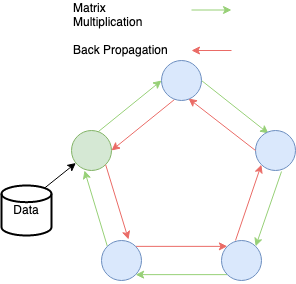
\includegraphics[width=0.3\textwidth]{ExampleNetwork}
    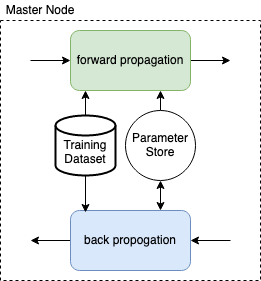
\includegraphics[width=0.3\textwidth]{masternode}
    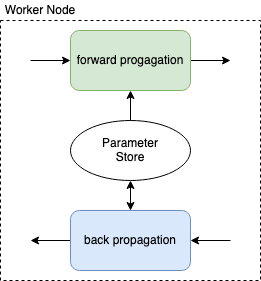
\includegraphics[width=0.3\textwidth]{SingleNode}
    \caption{
            Left: An example network of RingTMP. The green node being the master node and the blue nodes being the worker nodes.
            Centre: The architecture of the master node.
            Right: The architecture of the worker node.
        }
\end{figure}

My solution to address these issues raised above and a number of others is to
introduce a new model for distributed machine learning: \textit{RingTMP}.
RingTMP (Ring Topological Model Parallel) is a Ring Topological Model Parallel
distributed machine learning framework focusing on optimising Distributed
Stochastic Gradient Descent in low power hardware. This is a novel design
drawing in inspiration much research but particularly from the STRADS and
DistBelief machine learning frameworks. \cite{kim2016STRADS,Dean2012Distbelief}

As I have already alluded to this will take the form of a framework that will
operate on multiple machines which henceforth I will describe as nodes. Each
nodes contains a series of adjacent Deep Neural Network (DNN) layers. The
nodes are arranged in a ring. In the clockwise direction matrix multiplication
is performed and in the anticlockwise direction gradient descent through
backpropagation is performed. There are two kinds of nodes, master nodes and
worker nodes. Master nodes have direct access to the training data being input
into the Neural Network, whilst also performing operations on the data flowing
through the neural network. Worker nodes simply perform matrix multiplication
and backpropagation as it is directed via adjacent nodes. There is only one
master node per network and as many worker nodes as desired. 

These are the benefits my system will have over existing parameter server
architectures:
\begin{itemize}
    % \item RingTMP aims to reduce the time workers are idle to lower than the
    % parameter server model. This will manifest itself by distributing the work
    % between workers more proportionally, This means each computers resource is
    % used more efficiently and training should be faster per iteration.
    % \item The system will also not have a global parameter store, meaning there
    % will be no need for communication of weights across the network
    % \item As the node network has a ring topology not a star topology due the
    % lack of a need of a parameter server prevents one node getting flooded with
    % data each iteration. This isn't scalable, as when the workers increase so
    % does the data flooding the parameter server leading to bottlenecks. In
    % contrast the ring topology allows data to flow in lockstep, with no
    % bottlenecking
    % \item The convergence rate will be consistent across all nodes, and they are
    % all sharing a global problem rather than working on their own subproblems.
    % \item Because the convergence rate is the same across all nodes no scheduler
    % is necessary. Instead scheduling is managed in a decentralised manner via
    % communication with adjacent nodes.

    \item Workers will have less idle time, because the work will be distributed
    more proportionally between nodes. And computing resources will be used more
    efficiently.
    \item There will be less communication across nodes than the parameter
    server model as they will not need to send their local weights to the
    parameter server each iteration.
    \item There will also be a potential for larger communication bandwidth, as
    with RingTMP's ring topology only adjacent nodes need to communicate. While
    with a parameter server model every worker needs to communicate with the
    parameter server at the end of each iteration, which can lead to
    bottlenecking.
    \item The nodes require no scheduling as in some model parallel systems.
    Instead scheduling is managed in a decentralised manner via communication
    with adjacent nodes. This also makes the system more resilient, in the case
    of the scheduler crashing.
\end{itemize}

My aims more specifically for this project are to:
\begin{itemize}
    \item Create a prototype RingTMP framework and run it on multiple machines
    simultaneously.
    \item Create a parameter server model framework using the same tools that
    will run over multiple machines simultaneously.
    \item Show that RingTMP reduces the time workers are idle in comparison to
    the parameter server model.
    \item Demonstrate that RingTMP takes less overall power to run in comparison
    to the parameter server.
    \item Demonstrate that RingTMP is at least as scalable than a generic parameter
    server.
    \item Show that this solution can be as resilient as a parameter server
    model distributed neural network.
    \item Demonstrate that RingTMP can hold larger models on comparison to a
    standard parameter server, where each worker hold the whole model.
\end{itemize}
I will do this by running both systems on low power devices, then running
controlled experiments on them to measure their performance.



\subsection{Overview}
This document is split up into the following sections:
\begin{itemize}
 \item \textbf{Introduction} Current section. Introduce the project and its aims.
 \item \textbf{Background Research} Presents related research material and similar applications and areas.
 \item \textbf{Project Plan and Time Management} Gives an outline of my project timeline, methodology and assessment of risk.
 \item \textbf{Conclusion} Summary of previous sections.
 %\item \textbf{Section 4} Project plan and time management.
 %\item \textbf{Section 5} Summary of previous sections.
 %\item \textbf{Section 5} presents the design stages of the application.
 %\item \textbf{Section 6} outlines the application requirements and specifications
 %\item \textbf{Section 7} introduces the implementation and how they have been implemented.
 %\item \textbf{Section 8} describes the testing process
 %\item \textbf{Section 9} presents potential ideas for future work on the application.
\end{itemize}

% \subsection{Related Work}
% In order to understand the benefit this system will have over other Distributed
% Machine Learning Systems, one must first understand their different variations.
% While also understanding the benefits and drawbacks.
% \par

% There are two main variations with respect to the operation of the workers in
% parameter server model: 1) The parameter server has to wait for the last worker
% to be finished before it can calculate the new global parameters. much like the
% MapReduce algorithm. \cite{googlemapreduce2008} This is known as \textit{BSP}
% which stands for Bulk Synchronous Parallel Design.  2) The workers operate
% asynchronously constantly updating the parameter server, the parameter server
% calculating new global parameters periodically. \cite{Qirong2013SSP} This is known as
% \textit{ASP} which stands for Asynchronous Parallel Design. Whilst this
% method is the most common method of machine learning with many benefits, there
% are 3 key drawbacks:
% \begin{itemize}
%     \item The model sacrifices efficiency in either time or computation. Either
%     it must wait for all workers to be done each round, or redundant
%     computations must be made. \cite{Chilimbi2014ADAM}
%     \item when the parameter server is calculating the new global parameters the
%     workers are idle or otherwise computing on stale data. 
%     \cite{Verbraeken2020MLSurvey}
%     \item Each time the parameter server calculates a new global parameters,
%     these parameters must be broadcast to each worker simultaneously, consuming
%     vast network bandwidth. \cite{LI2014ParameterServers}
% \end{itemize}

% As has already been addressed frequently models can get so large that they can
% no longer feasibly be held within one worker. Therefore there are also
% variations with respect to how much of the model each worker operates on: 1) The
% model is segmented and split between worker. This is known as \textit{Model
% Parallelism} 2) The data is split between the workers which have their own full
% local models, but are synced with each other at periodic intervals. This is
% known as \textit{Data Parallelism} \cite{Xing2015Petuum} Though model
% parallelism shows promise it has its own set of drawbacks:
% \begin{itemize}
%     \item Often in model parallelism nodes do not communicate with each other,
%     this makes it performing algorithms such as Stochastic Gradient Decent
%     difficult as clusters of nodes are isolated.
%     \item some model parameters take more algorithmic iterations to converge
%     than others, so that they converges at the same rate, this means that some
%     nodes may be idle, not spreading the load equally or efficiently.
%     \cite{Dean2012Distbelief}
%     \item Because some parameters converge at different rates, a scheduler is
%     needed. However this in turn require more computational overhead and
%     communication and reduces iteration throughput. \cite{kim2016STRADS}
% \end{itemize}

% Taking all of these into consideration, I believe that I could design a system
% that avoids these limitations, therefore creating a efficient, scalable and
% resilient system.

% \par

% Each node has a 3 part structure.
% \begin{itemize}
%     \item The Parameter Store. This contains the parameters for this section of
%     the model. For the majority of the time its only accessed by elements within
%     the node.
%     \item The Multiplication Module. Reads the parameter server weights and
%     multiplies them with the matrix given by the previous node.
%     \item The Backpropagation Module. Takes the last layer of the previous node
%     and the parameters in the store. It uses them to calculate the new
%     parameters they are then placed in the Parameter Store.
% \end{itemize}

% The master node has the addition of being connected to the training dataset. A
% master node takes an single training example and its solution. It then send the
% example around the ring until it arrives back at the master node at which point
% the master node evaluates the decision the Neural Network has come to and begins
% the backpropagation progress along the way it came, in order to improve the
% model.



% produce diagram of node structure

% produce diagram of network structure

% talk about issue of communication vs computation




% \subsection{Problem}
% \todo{Address problems and what are the problems? \\ many solutions\\}
% T\lipsum[4]



